%
% einleitung.tex -- Beispiel-File für die Einleitung
%
% (c) 2020 Prof Dr Andreas Müller, Hochschule Rapperswil
%
% !TEX root = ../../buch.tex
% !TEX encoding = UTF-8
%
\section{Standardverfahren für Geodätenlinien
\label{geodaeten:section:Standardverfahren}}
\rhead{Standardverfahren für Geodätenlinien}

Lorem ipsum dolor sit amet, consetetur sadipscing elitr, sed diam
nonumy eirmod tempor invidunt ut labore et dolore magna aliquyam
erat, sed diam voluptua \cite{geodaeten:bibtex}.
At vero eos et accusam et justo duo dolores et ea rebum.
Stet clita kasd gubergren, no sea takimata sanctus est Lorem ipsum
dolor sit amet.

Lorem ipsum dolor sit amet, consetetur sadipscing elitr, sed diam
nonumy eirmod tempor invidunt ut labore et dolore magna aliquyam
erat, sed diam voluptua.
At vero eos et accusam et justo duo dolores et ea rebum.  Stet clita
kasd gubergren, no sea takimata sanctus est Lorem ipsum dolor sit
amet.


\section{Beispiele zum Standardverfahren}

%
% einleitung.tex -- Beispiel-File für die Einleitung
%
% (c) 2020 Prof Dr Andreas Müller, Hochschule Rapperswil
%
% !TEX root = ../../buch.tex
% !TEX encoding = UTF-8
%
\subsection{Kartesisch\label{geodaeten:section:Standardverfahren:Kartesisch}}
\rhead{Standardverfahren Beispiele}

\documentclass{article}
\usepackage{amsmath}
	
Für den kartesischen Raum mit dem metrischen Tensor 
\begin{equation}
g_{ij} = \begin{pmatrix} 
	1 & 0 \\ 
	0 & 1 
\end{pmatrix},
\end{equation}

wollen wir die Christophsymbole berechnen.
Die Christophsymbole sind gegeben durch,
\begin{equation}
\Gamma^i_{jk} = \frac{1}{2} g^{im} \left( \frac{\partial g_{mj}}{\partial x^k} + \frac{\partial g_{mk}}{\partial x^j} - \frac{\partial g_{jk}}{\partial x^m} \right),
\end{equation}

wobei $g^{im}$ die Inverse des metrischen Tensors ist.
Da der metrische Tensor $g_{ij}$ konstant ist und keine Abhängigkeit von den Koordinaten $\vec{x}$ hat, verschwinden alle Ableitungen.
Ohne weitere Berechnungen kann man also schließen, dass
\begin{equation}
\frac{\partial g_{ij}}{\partial x^k} = 0 .
\end{equation}

Somit ergeben sich alle Christophsymbole als null
\begin{equation}
\Gamma^i_{jk} = 0 .
\end{equation}

Denkt man an die Definition aus Abschnitt \ref{geodaeten:section:Standardverfahren}, macht dies durchaus Sinn.
Denn der Kartesische Raum ist nicht gekrümmt, weshalb keine Korrektur der Geraden notwendig ist.
Setzt man die Christophsymbole in die allgemeine Geodätengleichung ein erhält man mit $u^1 = x(t)$
\begin{equation}
\begin{aligned}
&\ddot{u}^1 + \Gamma_{ij}^1 \dot{u}^i \dot{u}^j = 0 \\
&\ddot{u}^1 + 0_{ij} \cdot \dot{u}^i \dot{u}^j = 0\\
&\ddot{u}^1 = 0 \\
&\ddot{x}(t) = 0
\end{aligned}
\label{geodaeten:equation:Standardverfahren:Kartesisch:x}
\end{equation}

und mit $u^2 = y(t)$

\begin{equation}
\begin{aligned}
&\ddot{u}^2 + \Gamma_{ij}^2 \dot{u}^i \dot{u}^j = 0 \\
&\ddot{u}^2 + 0_{ij} \cdot \dot{u}^i \dot{u}^j = 0 \\
&\ddot{u}^2 = 0 \\
&\ddot{y}(t) = 0 \qquad \qquad .
\end{aligned}
\label{geodaeten:equation:Standardverfahren:Kartesisch:y}
\end{equation}

Man sieht bereits, da die zweite Ableitungen in beide Dimensionen Null sind, handelt es sich bei dem Kürzesten Weg um eine Gerade.
Da sind wir froh, denn das macht durchaus Sinn.

Setzt man nun Zwei Punkte als Start und Endpunkt, kann man durch diese Nebenbedingungen eine konkrete Lösung erhalten.
Beispielsweise wollen wir den kürzesten Weg zwischen $P_A = (1,1)$ und $P_B = (3,5)$ berechnen. Wir integrieren die zweite Ableitung von x(t)

\begin{equation}
	\frac{d^2x}{dt^2} = 0 \Rightarrow \frac{dx}{dt} = c_1 
\end{equation}

, wobei $c_1$ eine Integrationskonstante ist. Durch erneutes Integrieren erhalten wir
\begin{equation}
\Rightarrow x(t) = c_1 \cdot t + c_2  .
\label{geodaeten:equation:Standardverfahren:Kartesisch:equation1}
\end{equation}

Wieder ist $c_2$ eine Integrationskonstante. 
Wir sehen, die Gleichung entspricht einer parametrierten Geradengleichung mit $c_2$ als Startwert für $x(0)$ und $c_1$ als Steigung von $x(t)$.

\begin{equation}
	P_A(x_1,y_1) \text{und} P_B(x_2,y_2)\\
	x(t) = (x_2 - x_1) \cdot t + x_1\\
	y(t) = (y_2 - y_1) \cdot t + y_1
\end{equation}

Da die Linie durch den Startpunkt gehen muss ist der Startwert bei $t=0$ bekannt als
 
\begin{equation}
	0 \cdot c_1 + c_2 = 1
\end{equation}
	
\begin{equation}	
	c_2 = 1 .
\end{equation}

Die Steigung $c_1$ kann mithilfe von Endpunkt und Startpunkt berechnet werden als

\begin{equation}
	c_1 = x_2 - x_1 \\ = 3-1 \\ = 2
\end{equation}

und damit ist die Lösung der Geodätengleichung in $x$ gleich

\begin{equation}
	x(t) = 2t + 1 .
\end{equation}


Analog für $y(t)$ ist [\ref{geodaeten:equation:Standardverfahren:Kartesisch:equation1}]
  
\begin{equation}
	\Rightarrow y(t) = c_3 \cdot t + c_4  .
\end{equation}

Die weiteren Gleichungen werden in $y(t)$ zu

\begin{equation}
	0 \cdot c_3 + c_4 = 1 
\end{equation}
 
\begin{equation}	
	c_4 = 1 .
\end{equation}

mit dem Einsetzen des Startwertes,

\begin{equation}
	c_4 = y_2 - y_1 \\=5-1 = 4
\end{equation}

mit der Steigung aus Sicht von $y$ und damit ist die Lösung der Geodätengleichung in $y$ gleich

\begin{equation}
	y(t) = 4t + 1 .
\end{equation}

\begin{figure}
	\centering
	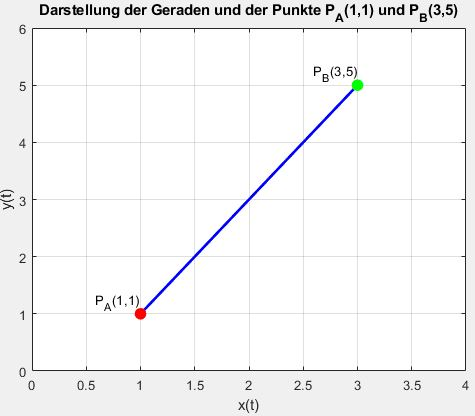
\includegraphics[width=10cm]{papers/geodaeten/Abbildungen/Standardverfahren/Kartesisch}
	\label{geodaeten:figure:Standardverfahren:Kartesisch:figure1}
	\caption{Darstellung der Kurve von x(t) und y(t) mit $t \in [0 , 1]$ Wie man sieht ist der kürzeste Weg von Punkt A zu Punkt B eine gerade.}
\end{figure}
%
% einleitung.tex -- Beispiel-File für die Einleitung
%
% (c) 2020 Prof Dr Andreas Müller, Hochschule Rapperswil
%
% !TEX root = ../../buch.tex
% !TEX encoding = UTF-8
%
\subsection{Zylinder\label{geodaeten:section:Standardverfahren:Zylinder}}
\rhead{Standardverfahren Beispiele}

Für die Zylinder Oberfläche mit konstantem $r$, mit dem metrischen Tensor 
\begin{equation}
	g_{ij} = \begin{pmatrix} 
		r^2 & 0 \\ 
		0 & 1 
	\end{pmatrix},
\end{equation}

wollen wir die Christophsymbole berechnen. 
Wie bei dem kartesischen Raum (Abschnitt \ref{geodaeten:section:Standardverfahren:Kartesisch}) werden alle Christophsymbole Null, da der metrische Tensor konstant ist.\footnote{
Auch in diesem Beispiel sind die Christophsymbole gleich Null.
Auf den ersten Blick könnte das verwirrend sein, da man bei einem Zylinder doch eindeutig eine Krümmung sieht.
Der Grund dafür ist, dass es sich bei dem Zylinder um eine extrinsische Krümmung handelt.
Die Zylinderoberfläche wird von außen zu einem Zylinder gekrümmt.
Abgerollt sieht man allerdings, dass die Oberfläche Flach ist.
Als weiteres Beispiel lässt sich berechnen, dass die Christophsymbole im Polarkoordinaten-Raum nicht gleich Null sind und daher eine Krümmung existiert, obwohl der Raum Flach erscheint.
Damit zeigt sich, dass die Intuition in diesem Fall täuschen kann.
}
Wir ersparen uns hier deshalb diese Rechnung.

Setzt man so $u^1 = \phi (t)$ und $u^2 = z(t)$ in die Geodätengleichung ein, so erhält man analog zu [\ref{geodaeten:equation:Standardverfahren:Kartesisch:x}]
\begin{equation}
	\ddot{\phi}(t) = 0
	\label{geodaeten:equation:Standardverfahren:Zylinder:phi}
\end{equation}

und dementsprechend gemäß [\ref{geodaeten:equation:Standardverfahren:Kartesisch:y}] 
\begin{equation}
	\ddot{z}(t) = 0 .
\end{equation}

Wählen wir $P_A(\phi_1 , z_1) = P_A(1 , 1)$ und $P_B(\phi_2 , z_2) = P_B(3 , 5)$ gleich wie in Abschnitt \ref{geodaeten:section:Standardverfahren:Kartesisch}, kennen wie bereits die Lösungen

\begin{equation}
	\phi(t) = 2t + 1 .
\end{equation}

\begin{equation}
	z(t) = 4t + 1 .
\end{equation}

Beim Zylinder ist jedoch interessant, dass es beliebige Lösungen für die Geodätengleichung gibt, da Die Winkelkoordinate Periodisch ist.
Durch Hinzufügen eines vielfachen von $2\pi$ macht die Kurve zusätzliche Runden um den Zylinder bevor es auf den Punkt $P_B$ trifft.
Dies ist zwar nicht die kürzeste Strecke, jedoch weder die Gleichung \ref{geodaeten:equation:Standardverfahren:Zylinder:phi} verletz noch der Punkt $P_a$ oder $P_B$ verfehlt.
Deshalb existieren sie als Scheinlösungen der Geodätengleichung.

Auch interessant ist, dass wenn die Oberfläche des Zylinders abgerollt auf eine Fläche dargestellt wird, ersichtlich ist, wie auch hier der kürzeste Weg eine Gerade ist.  

\begin{figure}
	\centering
	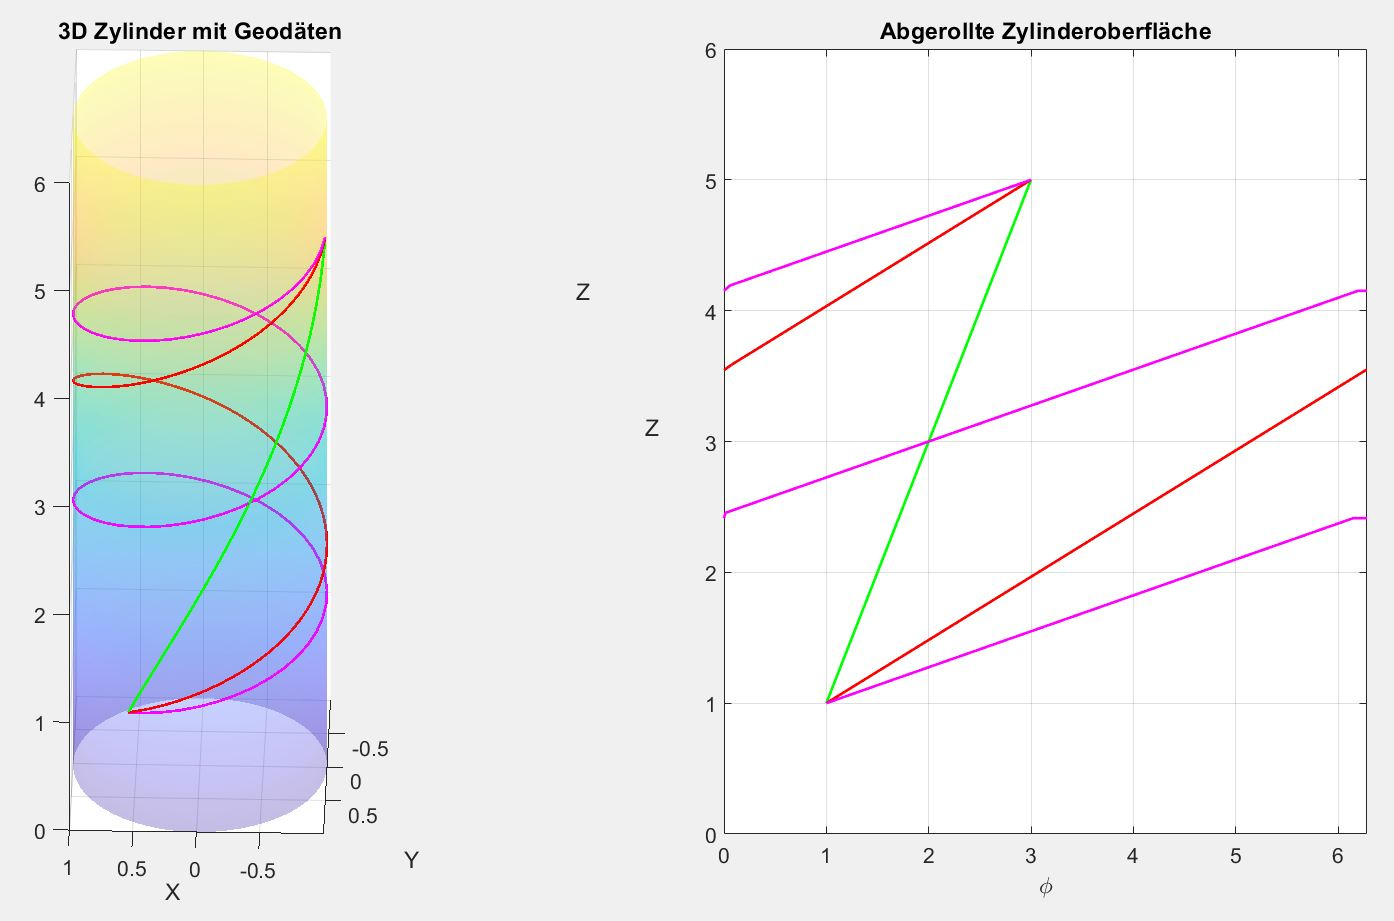
\includegraphics[width=14cm]{papers/geodaeten/Abbildungen/Standardverfahren/Zylinder}
	\caption{Darstellung der Geodätenlinien auf einem Zylinder und dessen abgerollte Oberfläche in einem 2D Plot mit Matlab}
	\label{geodaeten:figure:Linienelemente:Zylinder:figure1}
\end{figure}

%
% einleitung.tex -- Beispiel-File für die Einleitung
%
% (c) 2020 Prof Dr Andreas Müller, Hochschule Rapperswil
%
% !TEX root = ../../buch.tex
% !TEX encoding = UTF-8
%
\subsection{Kugel\label{geodaeten:section:Standardverfahren:Kugel}}
\rhead{Standardverfahren Beispiele}

Intuitiv erwarten wir, dass die Geodäten auf der Kugeloberfläche Grosskreise sind.
Ein Grosskreis ist der geradlinigste Weg zwischen zwei Punkten auf einer Kugel.
Dies kann man sich vorstellen, indem man zwei Nadeln in eine Kugeloberfläche steckt und einen Faden um die beiden Nadeln spannt.
Der Faden wird immer entlang eines Grosskreises verlaufen.
Tatsächlich folgen Flugzeuge auf Langstreckenflügen dieser Logik und fliegen entlang von Grosskreisen, um die kürzeste Strecke zwischen zwei Punkten auf der Erde zurückzulegen.
Wir möchten nun überprüfen, ob wir mit dem Standardverfahren tatsächlich zu dieser Lösung kommen.

Um dies zu tun, benötigen wir den bereits im vorherigen Abschnitt hergeleiteten metrischen Tensor für die Kugeloberfläche.
Dieser ist in Kugelkoordinaten $(\theta, \phi)$ gegeben durch
\begin{equation}
	g_{ij} = r^2 \begin{pmatrix}
		1 & 0 \\
		0 & \sin^2\theta
	\end{pmatrix}.
\end{equation}

Zuerst berechnen wir die Inverse des metrischen Tensors, da diese für die Berechnung der Christoffel-Symbol benötigt wird.
Der inverse Tensor $g^{ij}$ ist ergibt sich zu
\begin{equation}
	g^{ij} = \frac{1}{r^2} 
	\begin{pmatrix}
		1 & 0 \\
		0 & \frac{1}{\sin^2\theta}
	\end{pmatrix}.
	\label{geodaeten:equation:StaKugel:TensorInverse}
\end{equation}

Nun berechnen wir die partiellen Ableitungen des metrischen Tensors $g_{ij}$ in Bezug auf die Koordinaten $\theta$ und $\phi$.
Da $g_{11} = r^2$ und $g_{22} = r^2 \sin^2\theta$, erhalten wir
\begin{equation}
	\frac{\partial g_{11}}{\partial \theta} = 0, \quad \frac{\partial g_{11}}{\partial \phi} = 0, \quad \frac{\partial g_{22}}{\partial \theta} = 2r^2 \sin\theta \cos\theta, \quad \frac{\partial g_{22}}{\partial \phi} = 0.
	\label{geodaeten:equation:StaKugel:Ableitungen}
\end{equation}

\subsection{Christoffel-Symbole}
Mit den Ableitungen \eqref{geodaeten:equation:StaKugel:Ableitungen} und dem inversen Tensor $g^{ij}$ \eqref{geodaeten:equation:StaKugel:TensorInverse} können wir nun die Christoffel-Symbole berechnen durch
\begin{equation}
	\Gamma_{ij}^k = \frac{1}{2} g^{kl} \left( \frac{\partial g_{jl}}{\partial u^i} + \frac{\partial g_{il}}{\partial u^j} - \frac{\partial g_{ij}}{\partial u^l} \right),
\end{equation}
wobei $u^1 = \theta$ und $u^2 = \phi$.

Nach Einsetzen der Werte und Vereinfachung erhalten wir folgende nicht-verschwindende Christoffel-Symbole
\begin{equation}
	\Gamma_{12}^2 = \Gamma_{21}^2 = \cot\theta \quad \text{und} \quad \Gamma_{22}^1 = -\sin\theta \cos\theta.
\end{equation}

Anders als im Fall des Zylinders, wo der metrische Tensor konstant war, führt die Abhängigkeit des metrischen Tensors von der Koordinate $\theta$ zu nicht-verschwindenden Christoffel-Symbolen, welche die intrinsische Krümmung der Kugeloberfläche beschreiben.

Um diese Krümmung zu verstehen, betrachten wir die Bewegung eines Tangentialvektors auf der Oberfläche in Bezug auf die Basisvektoren.

Wird die Komponente des Vektors entlang eines Breitenkreises verändert, also in $\phi$-Richtung, führt das zu keiner Änderung der Vektorrichtung, da das Bogenmass von $\phi$ entlang eines Breitenkreises konstant bleibt.
Diese Bewegung beeinflusst die allgemeine Richtung des Vektors also nicht, was auch im metrischen Tensor reflektiert wird, der keinerlei Abhängigkeit von $\phi$ aufweist.

Andererseits führt eine Veränderung der Komponente entlang eines Längengrades, also in $\theta$-Richtung, zu einer Veränderung der Vektorrichtung.
Dies liegt daran, dass das Bogenmass von $\phi$ mit $\theta$ variiert: 
Je näher man den Polen kommt, desto kürzer wird der Bogen für eine gegebene Änderung von $\theta$, was die Gesamtrichtung des Vektors beeinflusst. 
Damit der Tangentialvektor seine ursprüngliche Richtung beibehält, müsste die Bewegung in der $\phi$-Richtung zunehmend verringert werden, je näher man den Polen kommt.

Diese Richtungsänderung des Vektors ist eine direkte Folge der intrinsischen Krümmung der Kugeloberfläche.
Die nicht-verschwindenden Christoffel-Symbole beschreiben genau diese Krümmung und geben an, wie sich die Richtung eines Vektors bei seiner Bewegung entlang der Oberfläche verändert.

\subsection{Geodätengleichung}
Mit den berechneten Christoffel-Symbolen können wir nun die Geodätengleichungen für die Kugeloberfläche aufstellen.

Die allgemeine Form der Geodätengleichung lautet
\begin{equation}
	\ddot{u}^k + \Gamma^k_{ij} \dot{u}^i \dot{u}^j = 0,
\end{equation}
wobei $u^k$ die Koordinaten darstellen, in diesem Fall $\theta$ und $\phi$.

Setzen wir die entsprechenden Christoffel-Symbole und Koordinaten in die Gleichungen ein, erhalten wir
\begin{equation}
	\begin{aligned} 
		0 &= \ddot{\theta} + \Gamma^1_{11} \dot{\theta} \dot{\theta} + 2\Gamma^1_{12} \dot{\theta}\dot{\phi} + \Gamma^1_{22} \dot{\phi} \dot{\phi} \\
		0 &= \ddot{\phi} + \Gamma^2_{11} \dot{\theta} \dot{\theta} + 2\Gamma^2_{12} \dot{\theta}\dot{\phi} + \Gamma^2_{22} \dot{\phi} \dot{\phi},
	\end{aligned}
\end{equation}
und weil einige der Christoffel-Symbole Null sind, vereinfachen sich die Geodätengleichungen schliesslich zu
\begin{align}
	0 &= \ddot{\theta} - \sin\theta \cos\theta \, \dot{\phi}^2 \\
	0 &= \ddot{\phi} + 2 \cot\theta \, \dot{\theta} \dot{\phi}.
\end{align}

Da $r$ lediglich ein Skalierungsfaktor ist, kürzt es sich in den Geodätengleichungen heraus. 
Die Geometrie wird allein durch die Winkelabhängigkeit bestimmt, sodass der Radius keinen Einfluss auf die Form der Geodäten hat.

Das Lösen der Geodätengleichungen ist oft aufwendig und schwierig, was numerische Ansätze erforderlich macht. 
Daher überprüfen wir durch Analyse, ob Grosskreise diese tatsächlich erfüllen und als Lösungen gelten.

\subsection{Äquator}
Betrachten wir die Geodätengleichungen für konstantes $\theta$, also entlang eines Breitengrads.
Für konstantes $\theta$ gilt $\dot{\theta} = 0$ und $\ddot{\theta} = 0$.
Setzen wir dies in die erste Geodätengleichung ein, so erhalten wir:
\begin{equation}
	0 = -\sin\theta \cos\theta \, \dot{\phi}^2.
\end{equation}
Die zweite Geodätengleichung vereinfacht sich zu $0 = \ddot{\phi}$, was zeigt, dass $\phi(t)$ linear in der Zeit variiert.
Diese erste Geodätengleichung wird nur für $\theta = \frac{\pi}{2}$ erfüllt, das heisst, nur für den Äquator.
Für alle anderen Breitengrade mit $\theta \neq \frac{\pi}{2}$ muss $\dot{\phi}$ gleich null werden, was bedeutet, dass es keine Bewegung in der $\phi$-Richtung gibt und somit keine Geodäte vorliegt.
Der Äquator, als einziger Breitengrad, erfüllt daher die Geodätengleichungen und ist ein Grosskreis.

\begin{figure}
	\centering
	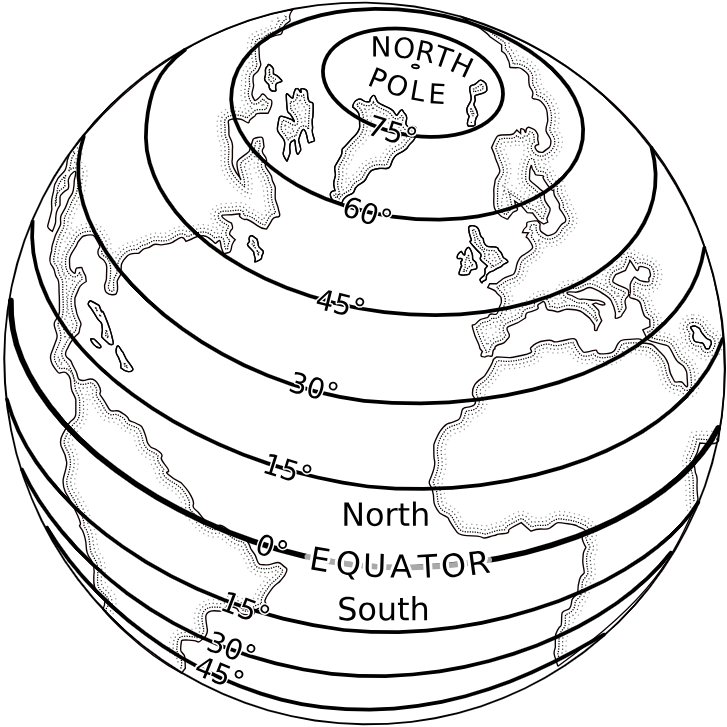
\includegraphics[width=1\linewidth]{papers/geodaeten/Abbildungen/Standardverfahren/StaKugelBreitengrade}
	\caption{Erdkugel mit Breitengrade und Äquator als Geodätenlinie}
	\label{geodaeten:figure:Standardverfahren:Breitengrade}
\end{figure}

\subsection{Längengrade}
Nun analysieren wir die Geodätengleichungen für konstantes $\phi$, also entlang eines Längengrads.
Für konstantes $\phi$ gilt $\dot{\phi} = 0$ und $\ddot{\phi} = 0$.
Setzen wir dies in die erste Geodätengleichung ein, erhalten wir:
\begin{equation}
	\ddot{\theta} = 0,
\end{equation}
was bedeutet, dass $\theta(t)$ linear in der Zeit variiert.
Die zweite Geodätengleichung wird ebenfalls trivial erfüllt, da $\dot{\phi} = 0$ und somit keine Beschleunigung in der $\phi$-Richtung vorliegt.
Damit sind alle Längengrade tatsächlich Geodäten.

Zusammenfassend konnten wir durch unsere Analyse zeigen, dass nur Grosskreise, wie der Äquator und die Längengrade, die Geodätengleichungen vollständig erfüllen und somit die wahren Geodäten auf der Kugeloberfläche darstellen.

Wir haben damit erfolgreich nachgewiesen, dass die Lösungen der Geodätengleichungen $\theta(t)$ und $\phi(t)$ zwangsläufig die Form von Grosskreisen annehmen müssen und dass die allgemeine Geodätengleichung diese Grosskreise korrekt als die Geodäten auf der Kugeloberfläche identifiziert.

\begin{figure}
	\centering
	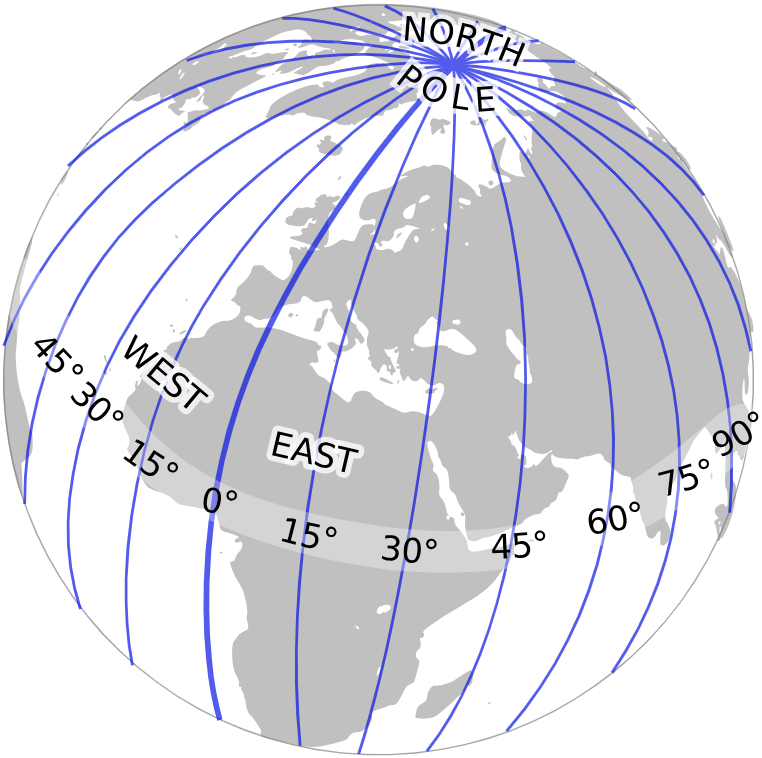
\includegraphics[width=1\linewidth]{papers/geodaeten/Abbildungen/Standardverfahren/StaKugelLaengengrade}
	\caption{Erdkugel mit Längengrade als Geodätenlinen}
	\label{geodaeten:figure:Standardverfahren:Laengengrade}
\end{figure}
